\chapter{基于数值计算的光子集成器件的发展趋势}\label{chap:1}

\section{光子集成与挑战}


\begin{figure}[!htbp]
    \centering
    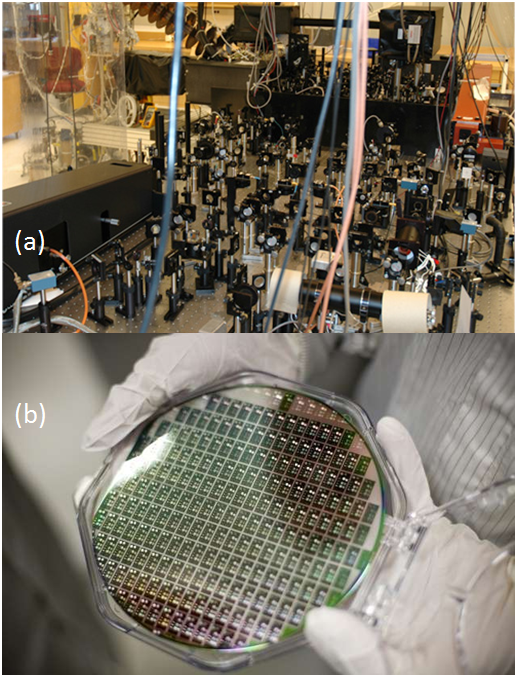
\includegraphics[width=0.60\textwidth]{1-1.png}
    \caption{光子集成目的,是将原本复杂繁多的光学实验器件(a),集成到紧凑的光子集成芯片(b)上,像电子集成电路一样,大规模普及应用,推动人类社会的发展。[{\color[HTML]{0000FF} 图片来源(a) Hau Laboratory (b)Dominick Reuter/MIT}]}
    \label{fig:1-1}
\end{figure}
%%%%%%%%%%%%%%%%%%%%%%%%%%%%%%%%%%%%%%%%%%%%%%%%%%%%%%%%%%%%%%%%%%%%%%%%%%%%%%%%%%%%%%%%%%%%%%%%%%%%%%%%%%%%%%%%%%%%%%



光子集成电路(Photonic Integrated Circuits, PIC),借鉴于电子集成电路的发展历程和技术思路,是一种集成了多种光子集成器件功能的芯片,可以在毫米级别的芯片尺寸下,如图1.1所示,集成多种光子器件,如滤波器、调制器、光放大器、激光器、光探测器等,通常在单晶硅\cite{Coldren2012Diode,Reed2005Silicon,Soref2007The}、氧化硅\cite{Takato1988Silica,Alberto2008Silica}、铌酸锂\cite{Toney2015Lithium}、或三五族化合物半导体\cite{Binetti2012Indium}的晶元表面上制备,实现复杂的光学功能。

光子集成电路的发展借鉴了电子集成电路的技术和思路,在过去的半个世纪,集成电路经历了快速发展,成为人类最伟大的发明和工业成就之一\cite{Lockwood2004Silicon},在极其紧凑的芯片上集成数亿万个的纳米晶体管,实现高性能的微处理器或大容量的存储芯片等,极大推动了社会进步,改变了人类的生活方式。跟电子集成电路的迅猛发展相比,光子集成电路的发展则较为缓慢,主要有以下的技术限制:

一、电子集成电路可以通过纳米量级的铜线实现晶体管等电子器件的连接,具有极高的便捷性和集成度。而片上的光子集成电路则是通过光波导相连,受限于光的波长,波导尺寸和器件尺寸一般为微米以上量级,且波导不能进行剧烈的弯曲。在一定程度上限制了光子集成芯片的集成度,从而光子芯片的生产成本很难下降。

二、波导与光纤的耦合器之间的光学耦合,相比电子芯片的连接器更为严苛。波导传输与器件的功能实现的存在不可避免的光能量损耗。相比可以通过晶体管放大的电信号\cite{Wissem2014Bridging,Miller2010Optical}。片上集成的光放大器的较为复杂,成本较高,减少光的能量损耗则是更为经济适用的突破方向。减少光器件的损耗需要提高现有的光子器件设计方法。

三、一些片上的光子器件很难实现微型化,如用于密集波分复用DWDM的阵列波导光栅AWG等

有了上述的技术限制,光子集成电路很难达到电子集成电路的复杂程度和低成本。但是,以磷化铟InP为主的三五族化合物半导体的光子集成芯片,凭借其材料的优势,极大地推动了光通信应用的发展,如集成的多路光收发芯片等,在超算和数据中心中应用,包含DFB激光器,高速光调制器、光探测器和光滤波器等。\cite{Kish2011Current}

仍然需要通过器件设计的优化,设计出更多更紧凑的光子器件,实现更低的损耗和更高的性能,以提升光子集成电路的功能和降低芯片的制造成本。使得光子集成芯片,可以像电子集成芯片实现更为广泛的应用。\cite{Reed2008Silicon}


\section{计算机运算能力突飞猛进?}

\begin{figure}[!htbp]
    \centering
    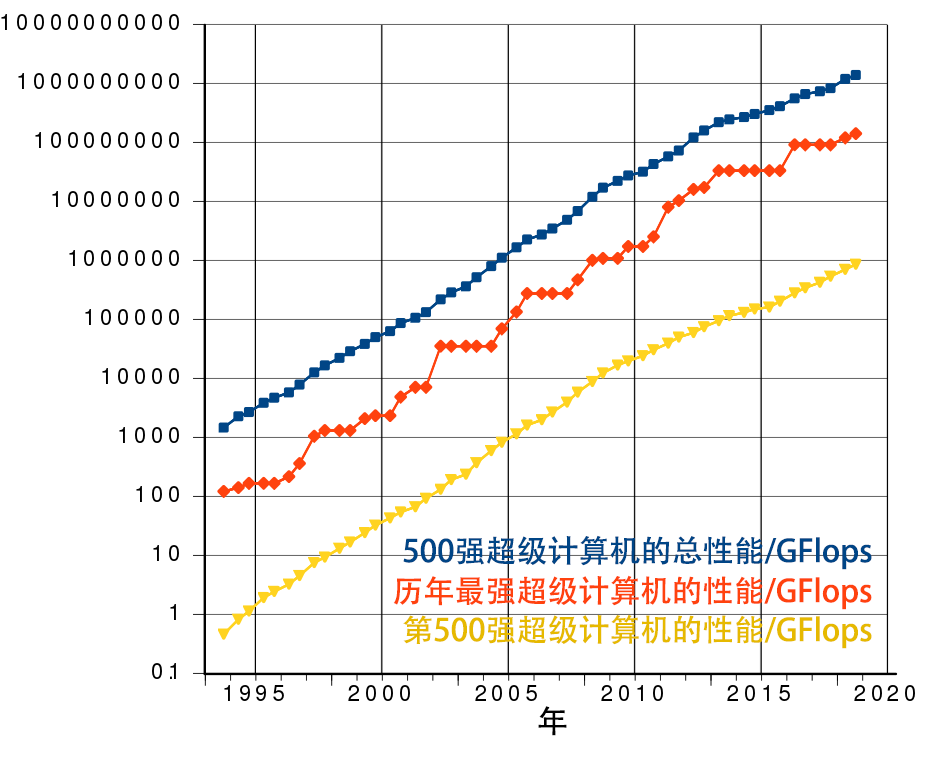
\includegraphics[width=1\textwidth]{1-2.png}
    \caption{评测结构TOP500统计的全球前500强超级计算机的浮点性能的发展规律,其中超算的浮点性能以每12年翻1000倍的速率指数增长,为光子集成器件的纯数值设计提供了可能。[{\color[HTML]{0000FF} 图片来源:TOP500}]}
    \label{fig:1-2}
\end{figure}
%%%%%%%%%%%%%%%%%%%%%%%%%%%%%%%%%%%%%%%%%%%%%%%%%%%%%%%%%%%%%%%%%%%%%%%%%%%%%%%%%%%%%%%%%%%%%%%%%%%%%%%%%%%%%%%%%%%%%%
自计算机诞生以来,计算机的计算能力有着令人瞩目的增长。以超算为例,如图1.2为有美国田纳西州大学和美国国家能源研究科学计算机中心NERSC牵头的超算评测机构TOP500通过LINPACK测试(每半年评测一次)的世界上500强的超级计算机的浮点运算性能的发展趋势,其中在2013年到2016年连续六次世界排名第一的,由国防科技大学设计建造的天河二号超级计算机,达到了33.86 PetaFlop/s的实测双精度浮点运算速度,即每秒能实现 $3.3\times10^{16}$次双精度浮点计算。而截止2019年,世界最强超算为美国橡树岭国家实验室的Summit超级计算机,其实测浮点性能比天河二号更快,达到143.5 PetaFlop/s。由于超级计算机的计算能力通常是普通科研用高配置工作站的$10^4\sim 10^5$倍,发展规律也可近似等效为一般科研计算机的发展规律。\cite{top500}

从图1.2的发展趋势来看,超级计算机的计算性能呈现出每十二年增长1000倍的指数增长趋势:自1996年500强中首次出现TeraFlop级的超级计算机,到2008年首次出现PetaFlop级的超级计算机,通过趋势的预测,到了2020年将会有ExaFlop级别的超算诞生。

计算机运算能力的空前发展,给光子集成器件的设计带来了前所未有的发展机遇,可以通过更高精度、更快速的数值运算,可以实现功能更加全面、器件更加紧凑的光子器件的设计。

\begin{figure}[!htbp]
    \centering
    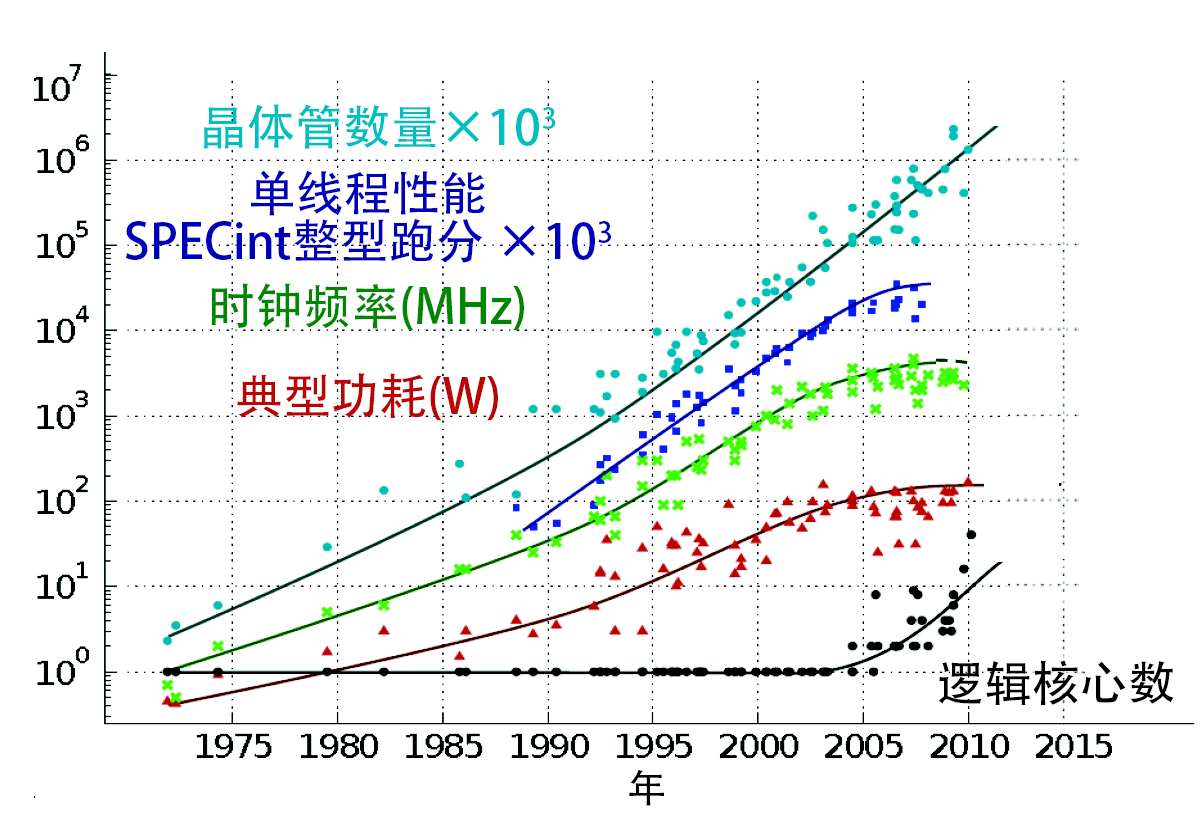
\includegraphics[width=1\textwidth]{1-3.png}
    \caption{摩尔定律驱动下,晶体管数量呈现指数式增长,是依靠逻辑核心数量的提升。随着集成电路铜导线的物理带宽的限制,处理器的时钟频率提升趋于平缓,单线程性能趋于饱和,迫切需要研究更加高效的光学优化算法。[{\color[HTML]{0000FF} 图片来源:Karl Rupp}]}
    \label{fig:1-3}
\end{figure}
%%%%%%%%%%%%%%%%%%%%%%%%%%%%%%%%%%%%%%%%%%%%%%%%%%%%%%%%%%%%%%%%%%%%%%%%%%%%%%%%%%%%%%%%%%%%%%%%%%%%%%%%%%%%%%%%%%%%%%

超级计算机的的迅速崛起,离不开微型处理器的摩尔定律式发展,如图1.3所示为奥地利维也纳工业大学计算机专家的Karl Rupp等人整理的近40年的微型处理器发展情况。

自1980年代微型计算机进入消费者市场,强大又便宜的计算机给行业带来了巨大的变化,巨大的社会需求和市场竞争也促进了集成电路行业的迅猛发展。其中,计算机核心的微处理器的运算能力从战后的每24个月翻一番,到1980年代的18个月翻一番,到1990年代的每12个月翻一番。\cite{42years}

图1.3为计算机微处理器的发展趋势。可以看到,虽然微处理器的晶体管数量仍旧保持强劲的指数增长趋势。然而,随着微处理器中金属铜导线的物理带宽限制,微处理器的芯片的时钟频率开始趋于饱和。依赖于更加智能的功耗控制和动态的时钟频率调节的等技术,微处理器的单核心的性能虽在不断增长,但也逐渐趋于平缓。单核心性能的不断增长,说明了单核心性能在实际应用中具有重要意义,相比多核心的复杂算法,需要进行繁杂的多核心资源调度和算法优化,单核心性能具有便捷和高效的作用。\cite{42yearsgit}

从另一个角度,单核心性能的增长缓慢,也说明了不能寄希望于简单粗暴的数学计算来进行光学计算和优化。需要发展更加可靠的并行计算算法,或者发展更加智能高效的光学计算算法。

\section{光子器件的仿真趋势}

\begin{figure}[!htbp]
    \centering
    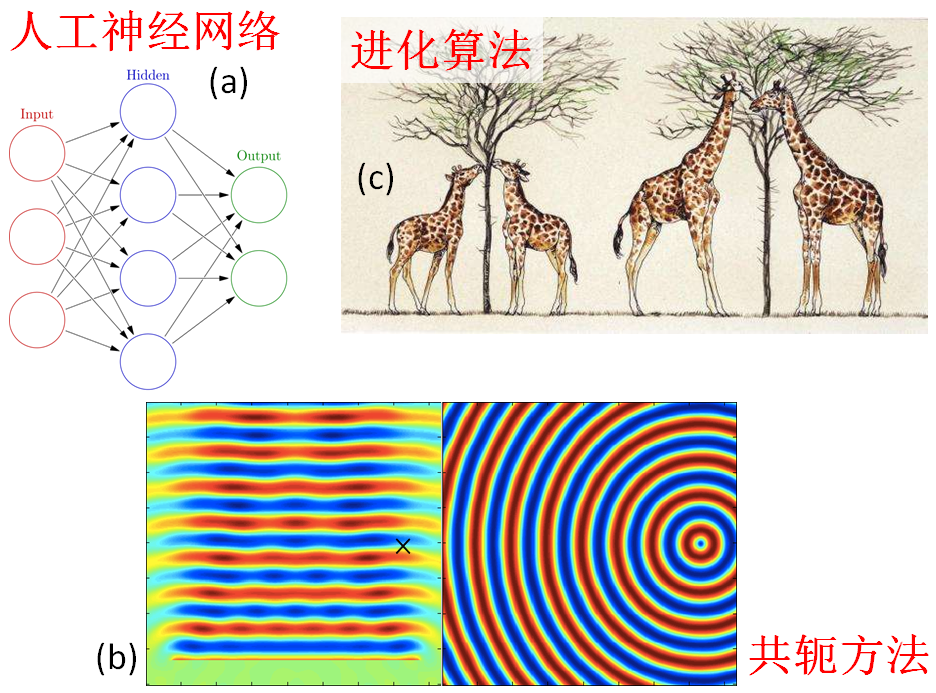
\includegraphics[width=1\textwidth]{1-4.png}
    \caption{较为主流的光学设计方法,有依靠大样本学习拟合的人工神经网络(a)、通过计算演化梯度的共轭办法(Adjoint method)(b)、以及通过自适应、自学习寻优的进化算法(c)。[{\color[HTML]{0000FF} 图片来源(b) IAC Publishing (c) Yablonovitch Group, UC Berkeley}].}
    \label{fig:1-4}
\end{figure}
%%%%%%%%%%%%%%%%%%%%%%%%%%%%%%%%%%%%%%%%%%%%%%%%%%%%%%%%%%%%%%%%%%%%%%%%%%%%%%%%%%%%%%%%%%%%%%%%%%%%%%%%%%%%%%%%%%%%%%
计算能力的迅猛发展,推动了光学计算和优化的发展。如图1.4所示,近几年,常用的光学计算和优化的方法主要有通过大样本学习和非线性拟合的人工神经网络、用于计算演化梯度下降的共轭方法(Adjoint method),以及自适应、自学习寻优的进化算法等。

其中,人工神经网络可以通过大量的数据案例进行学习和非线性拟合分析,获得光学器件的变量参数与器件性能指标之间隐含的深层关系,通过数据挖掘,寻找和预测新的器件设计参数。\cite{Liu2017Training}

共轭方法通过引入光学优化目标函数的背向传播(back propagation),通过正向传播和共轭背向传播的相干关系,实现演化梯度的计算,便于更快更好的实现目标函数的优化。\cite{Vu2013Nanophotonic,Lu2013Objective,Molesky2018Outlook}

而进化算法的方案,则是通过自适应、自学习的变量迭代,逐渐进步的方式,实现逐步更好的光学设计,常见的进化算法主要有借鉴生物规律的法则的遗传算法等。

通过上述的算法,可以在一维、二维、三维光器件设计中,设计并优化的光学器件,相比传统设计的光学器件具有更加明显的优势。


\begin{figure}[!htbp]
    \centering
    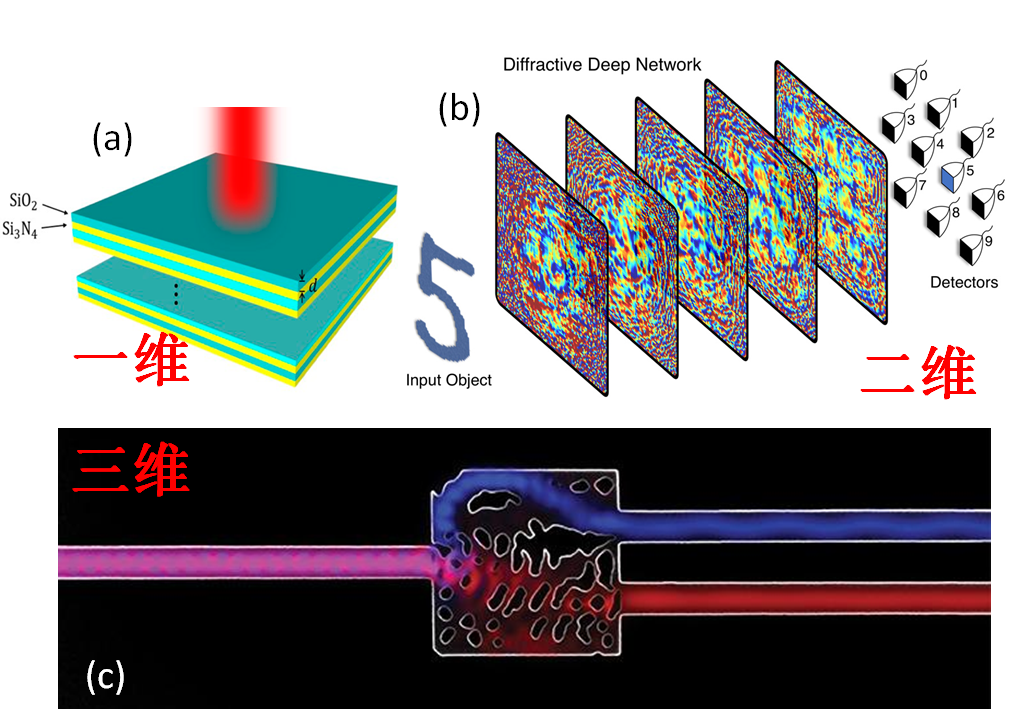
\includegraphics[width=1\textwidth]{1-5.png}
    \caption{通过光学优化算法,可以在一维、二维、三维的光学上进行优化设计。如通过深度神经网络优化氧化硅/氮化硅的一维光学薄膜(a);通过共轭办法优化的二维衍射元件,形成用于加速文字和图像识别的衍射深度网络(b);通过目标优先(objective-first)的共轭方法设计的三维1310/1550nm波长复用集成光子器件。本论文中,三维光子集成器件为研究的重点。\cite{Liu2017Training,Xing2018All,Piggott2015Inverse}}
    \label{fig:1-5}
\end{figure}
%%%%%%%%%%%%%%%%%%%%%%%%%%%%%%%%%%%%%%%%%%%%%%%%%%%%%%%%%%%%%%%%%%%%%%%%%%%%%%%%%%%%%%%%%%%%%%%%%%%%%%%%%%%%%%%%%%%%%%

上述算法的设计涵盖了一维、二维、三维光学应用的计算与优化。一维的光学设计主要是光学薄膜或量子阱设计等,如图1.5a所示,美国威斯康星大学的Dianjing Liu等人,通过75万组数据的深度人工神经网络的机器学习,找到氧化硅和氮化硅交替生长的光学薄膜和对应的透射谱之间的非线性网络关系,通过深度神经网络的拟合和预测,可以设计出具有任意透射谱效果的光学薄膜。\cite{Liu2017Training}

二维的光学设计,主要是二维衍射元件的设计,如图1.5b所示,加州大学洛杉矶分校的Xing Lin等人,通过计算并3D打印多层的光学衍射介质板,构建了一个衍射神经网络系统,实现了手写数字和图像的自动识别。光学的多层衍射系统可以成为人工神经网络的加速平台,实现更低功耗更高性能的多层衍射神经网络系统。\cite{Xing2018All}

三维的设计包括片上的超材料硅光子器件设计,如图1.5c所示的美国斯坦福大学的Alexander Y. Piggott等人,通过基于目标优先的共轭方法梯度下降进行目标函数的优化,反向设计了器件尺寸5×5$\mu$m$^2$的C+O波段的波长复用器件。\cite{Piggott2015Inverse}

其中,三维的超材料硅基光子器件的设计,有利于解决当前光子集成芯片所面临的问题,具有集成度高、器件紧凑,制备简单高效的特点,也是本论文研究的重点。\cite{Staude2017Metamaterial,Yang2015On}

\begin{figure}[!htbp]
    \centering
    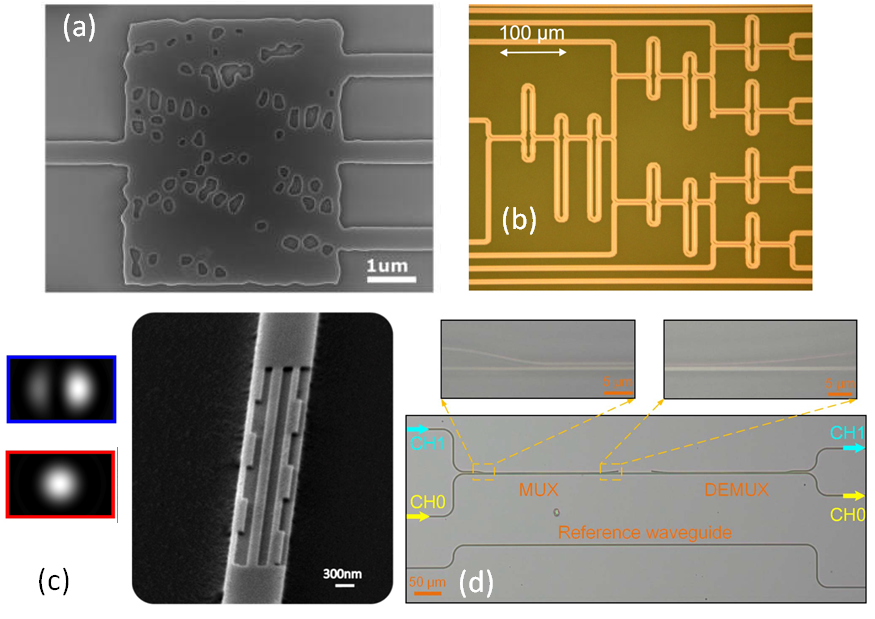
\includegraphics[width=1\textwidth]{1-6.png}
    \caption{两个简单案例,说明了超材料光子器件的尺寸优势。(a) 斯坦福大学设计的三通道40nm间隔粗波分复用(CWDM)光子集成器件,器件尺寸为4×5$\mu$m$^2$。(b) IBM设计的传统的基于级联马赫-曾德尔八通道5nm间隔的CWDM器件,器件尺寸为400×500$\mu$m$^2$。(c) 希伯来大学设计的波导集成TE0-TE1模 式转换器,器件长度仅20$\mu$m。(d) 中科院上海微系统与信息技术研究所设计的传统基于方向耦合器的TE0-TE1模式转换器,器件长度为260$\mu$m。\cite{Su2017Inverse,Folkert2013Cascaded,Ohana2016Dielectric,Jing2015Broadband}}
    \label{fig:1-6}
\end{figure}
%%%%%%%%%%%%%%%%%%%%%%%%%%%%%%%%%%%%%%%%%%%%%%%%%%%%%%%%%%%%%%%%%%%%%%%%%%%%%%%%%%%%%%%%%%%%%%%%%%%%%%%%%%%%%%%%%%%%%%

基于计算优化的超材料光子器件,在近些年成为研究的热门。设计的超材料光子器件,相比传统的器件,具有尺寸紧凑,效果显著的特点。如图1.6,们列举了两个简单的案例,说明超材料光子器件巨大的尺寸优势。

如图1.6a的由美国斯坦福大学的Alexander Y. Piggott等人,通过目标优先的共轭方法,通过计算物质结构的演化梯度反向设计,得到的基于硅的三通道40nm间隔CWDM光子器件,器件尺寸仅为4×5$\mu$m$^2$,约2dB的插入损耗和10dB的串扰抑制比,具有初步的应用可行性\cite{Su2017Inverse}。相比之下,瑞士IBM苏黎世研究院的Folkert Horst等人设计的基于级联马赫曾德尔干涉仪的CWDM的器件相比,如图1.6b,器件尺寸为400×500$\mu$m$^2$,插入损耗约为1.6dB,18dB的串扰抑制比\cite{Folkert2013Cascaded}。可以看到,原本需要数百微米尺寸的光子器件,可以通过数微米大小的尺寸来初步实现,具有很大的意义。

第二个案例,以色列希伯来大学的David Ohana 等人,通过在纳米尺度的波导上制备的超材料器件,通过20$\mu$m的单模硅波导长度,实现了TE0到TE1模式的模式转换,插入损耗约为0.55dB,TE1与TE0的模式抑制比为12.7dB \cite{Ohana2016Dielectric};相比之下,而与中国科学院上海微系统与信息技术研究所的Jing Wang等人设计的传统的基于方向耦合器的TE0-TE1模式复用/转换器,其器件的长度为260$\mu$m,插入损耗<0.1dB,TE1与TE0的模式抑制比>20dB,如图1.6d \cite{Jing2015Broadband},虽然器件性能较差,但器件尺寸同样相差一个数量级。

实际上,三维的超材料光子器件能实现更多的光学功能。通过调研、整理,将目前发表的超材料光子器件的应用场景进行归类,有折射率工程(index-engineering)、模式转换、波长复用、群速度工程、偏振复用、特殊波束发射等功能。

如图1.7a所示,德克萨斯大学奥斯丁分校的Yang Zhang等人,通过在传统的基于布洛赫波的光交叉阵列的两侧,制备了亚波长超材料的微结构,通过折射率工程实现了包层折射率的提升,并将传统的光交叉阵列的损耗降低到-0.02dB/crossing的程度,且交叉串扰<-40dB。\cite{Yang2013Ultralow}

如图1.7b所示,香港中文大学的Zejie Yu等人,通过遗传算法优化的像素超材料,实现了1×4$\mu$m的宽带硅波导的TE和TM偏振模式转换器,在紧凑的器件尺寸下,实现了-0.7dB的最小插入损耗和157nm的1dB带宽。\cite{Cui2017Genetic}

如图1.7c所示,斯坦福大学的Alexander Y. Piggott等人,通过目标优先(objective-first)的共轭方法设计的O波段和C波段的波长复用光子器件,器件尺寸小于3×3$\mu$m$^2$,波长串扰<11dB,带宽>100nm。\cite{Piggott2015Inverse}

如图1.7d所示,渥太华大学的Przemek J. Bock通过亚波长光栅波导(Sub-Wavelength Grating)的群速度工程,实现了超C波段的100nm光谱波段下实现了TE和TM模式的群折射率恒定为$\sim$1.5,实现了随心所欲的群速度调控。\cite{Bock2010Subwavelength}

如图1.7e所示,犹他大学的Bing Shen等人通过非线性的优化算法实现了2.4×2.4微米的超材料的偏振复用器,实现了TE、TM模式的复用。\cite{Bing2015An}

如图1.7f所示,深圳大学的Zhenwei Xie等人通过反向设计的±1阶OAM光束发射器,插入损耗约-5dB,带宽超过200nm。\cite{Xie2018Ultra}

综上所述,通过数值计算设计、优化的超材料光子器件具有较高的设计潜力,丰富的自由度和应用前景,因此,本论文主要设计紧凑的光子器件,尝试在光栅耦合器、层间耦合器和光子长通滤波器领域实现应用,丰富超材料的光子器件库,为提高光子集成度和降低光子芯片成本提供可参考的、有价值的技术方案。\cite{Zheludev2012From,Yang2015On,Shen2016Increasing,HongnanMetamaterial}

\begin{figure}[!htbp]
    \centering
    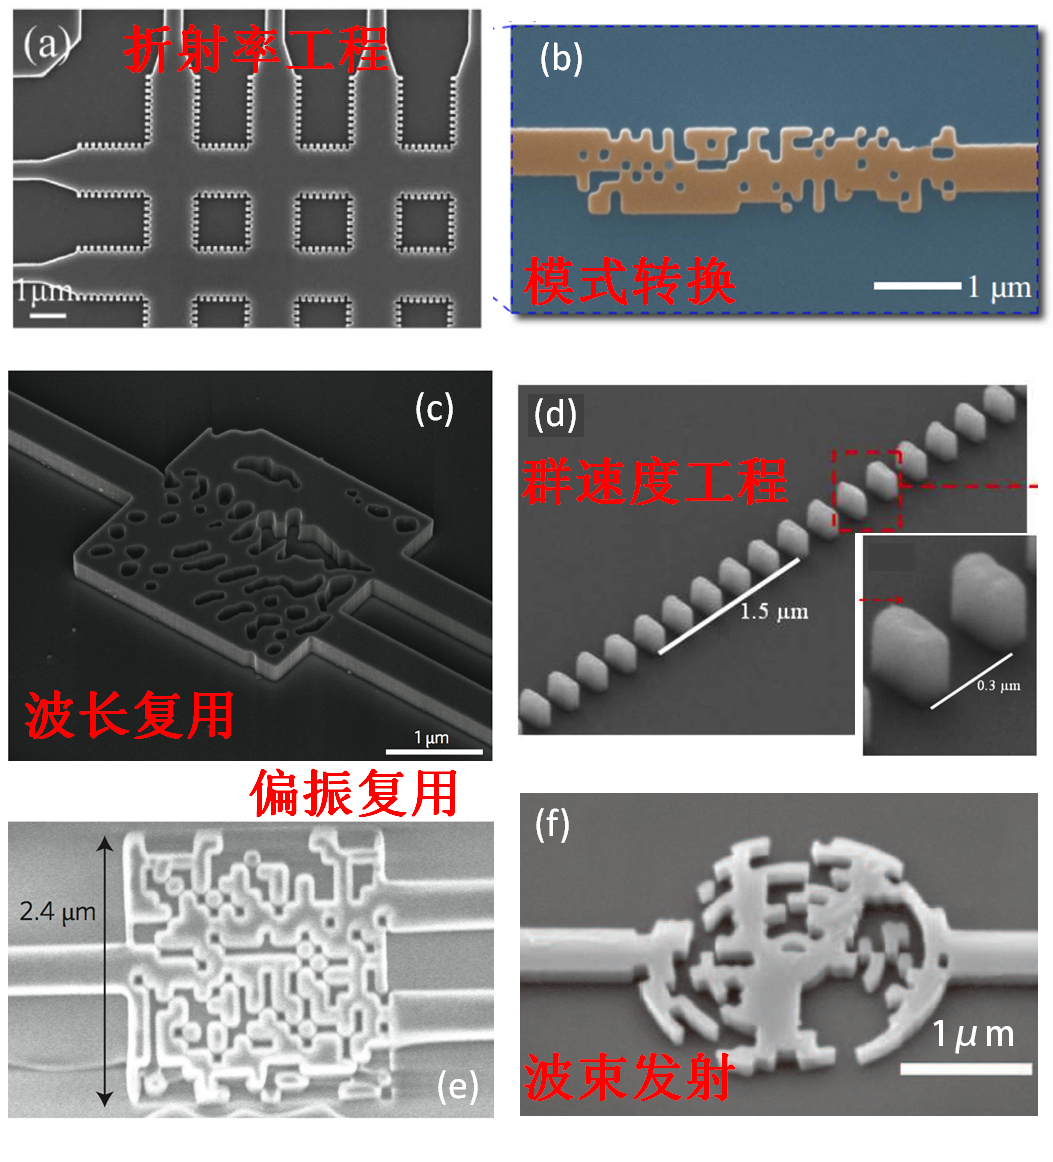
\includegraphics[width=1\textwidth]{1-7.png}
    \caption{超材料集成光子器件的案例,可以实现丰富的功能。如(a)折射率工程、(b)波导模式转换、(c)波长复用、(d)群速度工程、(e)偏振复用、(f)特殊波束表面发射等\cite{Yang2013Ultralow,Cui2017Genetic,Piggott2015Inverse,Bock2010Subwavelength,Bing2015An,Xie2018Ultra}}
    \label{fig:1-7}
\end{figure}
%%%%%%%%%%%%%%%%%%%%%%%%%%%%%%%%%%%%%%%%%%%%%%%%%%%%%%%%%%%%%%%%%%%%%%%%%%%%%%%%%%%%%%%%%%%%%%%%%%%%%%%%%%%%%%%%%%%%%%
